\documentclass[11pt,a4paper]{article}
\usepackage[margin=1in]{geometry}
\usepackage[T1]{fontenc}
\usepackage{lmodern,microtype,amsmath,amssymb,booktabs,tabularx,graphicx}
\usepackage{xurl}
\usepackage[hidelinks]{hyperref}
\setlength{\emergencystretch}{2em}
\renewcommand{\thesection}{S\arabic{section}}
\renewcommand{\thetable}{S\arabic{table}}
\renewcommand{\thefigure}{S\arabic{figure}}
\title{Supplementary Material\\\large Why Should They Expand? Computational Growth, Resource Sufficiency, and Conditional Interstellar Expansion}
\author{Hyeonjun Joo}
\date{12 October 2026}
\hypersetup{pdfsubject={CITH v7.3 supplementary material}}
\begin{document}
\maketitle
\section{Numerical checks and concavity certificates}
Corner classifications are determined analytically, without optimizing
budget shares. A separate implementation also checks every stored
optimizer output. For budget-share vectors $v$ in the unit simplex, let
\[
 G(v)=\max_j[\nabla U(v)]_j-\nabla U(v)\cdot v.
\]
For any other feasible share vector $v'$, concavity gives
$U(v')-U(v)\leq\nabla U(v)\cdot(v'-v)\leq G(v)$, since
$\nabla U(v)\cdot v'$ is a convex combination of gradient entries.
This proves the objective-gap bound. The reported normalized certificate
is $\max\{0,G(v)\}/(1+|U(v)|)$; truncation removes only negative
floating-point round-off. It is not an exact-arithmetic optimizer proof.

The audit reconstructs the objective and gradient directly from the
frozen parameters and stored budget shares. It does not import the
original model. All 14,336 stored solutions are feasible and pass the
$2\times10^{-6}$ normalized-gap tolerance. The largest observed
normalized gap is $1.32370\times10^{-6}$, and the largest absolute objective
reconstruction difference is $3.55271\times10^{-15}$.
All exact corner classifications match the archived flags. At every
finite positive productivity threshold, the code checks
$a=a_{\mathrm{crit}}(1-10^{-6})$ and
$a=a_{\mathrm{crit}}(1+10^{-6})$, for 11,002 tests in total.

A separate scalar optimizer checks the pure-computation allocation at
101 budgets, with maximum objective discrepancy
$1.81899\times10^{-12}$. The two-period construction is checked at
201 external-yield settings against a joint optimization
in $(x_1,z_2,x_2)$ with explicit second-period budget feasibility.
Two initial conditions are used for each joint optimization.
The maximum absolute objective difference is $1.49036\times10^{-12}$.
The reproduced transition is $g_X=0.4091479213$; at $g_X=2$,
$x_1=3.7559168566$ and $B_2=9.7606503419$.
The script also rechecks all four support paths, the finite-depth lemma,
the nonconcave negative control and the fixed/random-origin silence
probabilities. It does not rerun the original Monte Carlo population
simulations or the removed settlement benchmark.

\section{Generator provenance and frozen-input reproduction}
The original environment record gives Python~3.13.5, NumPy~2.3.5 and
SciPy~1.17.0. The normalized call is
\begin{verbatim}
u = scipy.stats.qmc.Sobol(
    d=14, scramble=True, seed=20260905
).random_base2(m=10)
\end{verbatim}
The original source writes the same dimensions and power through its
variables \texttt{len(NAMES)} and \texttt{power}. The effective bit depth
is 30, with no optimization, skipping or thinning. The archive stores
both the unit points and transformed parameter rows. The reference
file's SHA-256 is
\begin{quote}\small\ttfamily
\nolinkurl{ce45ecd0435f2abf834445957db369d1d4a5bc28e9c4e7b686561df50a14194b}
\end{quote}
Array hashes use contiguous row-major little-endian float64 bytes and
are recorded in \path{results/archive_audit.json}.

\begin{table}[htbp]\centering
\caption{Same-version generator-interface comparison. All calls use
SciPy~1.17.0, $d=14$, $m=10$, scrambling and the same integer seed.
``Same points'' means bit-for-bit equality with the archived unit array.}
\begin{tabular}{@{}lcrr@{}}\toprule
Interface & Same points & Reference & Perfect substitution\\\midrule
\texttt{seed=20260905} & Yes & 219 & 527 \\
\texttt{rng=20260905} & No & 208 & 530 \\
\bottomrule\end{tabular}
\end{table}
The \texttt{seed} call reproduces the unit points exactly. The transformed
parameters differ in some last bits, with maximum relative difference
$2.21773\times10^{-16}$, without any classification change. Both keyword paths
instantiate NumPy Generator/PCG64 objects in the environment tested; it
would therefore be inaccurate to describe the observed difference simply
as RandomState versus Generator. With \texttt{seed=20260905}, the archived unit points are reproduced
bit for bit under SciPy~1.17.0 and 1.18.1;
\texttt{rng=20260905} yields a different scramble, with 208
instantaneous and 530 perfect-substitution inward corners. The frozen
arrays, not the seed alone, define the reference experiment.

Eight further scrambles for each of log-uniform and linear-uniform
marginals are regenerated and agree with the archived measure-sensitivity
results. These checks assess the selected mathematical design, not an
extraterrestrial sampling distribution.

\section{New mathematical examples and executable outputs}
\subsection*{Growing budgets and persistence}
For the one-direction example $r=0.1$, $S=0.001$, $d_0=2$ and fixed
external price $p=1$, the required logarithmic price is $H+A/a$.
The equation $H(B)=1$ has the numerical solution $B_\dagger\simeq189.490600549$.
At $B\geq B_\dagger$ no finite productivity can meet the corner
test with these fixed coefficients. Table~\ref{tab:growth} also checks
constructive paths satisfying the exact condition. In the price-growth
path, $p(B)=2H(B)$ and $a(B)=B+A(B)/H(B)$. In the residual-decay
path, $p=1$, $S(B)=1/[2(1+B)\ln(1+B)]$, and
$a(B)=B+2A(B)$. All points are deliberately constructed examples.
\begin{table}[htbp]\centering
\caption{Growth-path checks. The last two columns report required price
divided by actual price for the two constructive paths; values below
one pass the corner test.}\label{tab:growth}
\begin{tabularx}{\textwidth}{@{}r*{4}{>{\raggedleft\arraybackslash}X}@{}}\toprule
$B$ & $H$ (fixed $S$) & Required $p$ at $a=100$ & Price-growth path & Residual-decay path\\\midrule
10 & 0.026377 & 0.037597 & 0.904830 & 0.616390 \\
100 & 0.466127 & 0.569147 & 0.590504 & 0.585521 \\
1000 & 6.915664 & 7.936684 & 0.507275 & 0.583503 \\
\bottomrule\end{tabularx}\end{table}

\subsection*{Curvature trichotomy}
For $B=10$, $r=0.1$, $S=0.001$, $d_0=2$ and $p=1$, the
computed thresholds are listed in Table~\ref{tab:curvature}.
Global scalar optimizations use
\[
 U(x)=F_\eta\big(1+a\ln(1+10-x)+0.1x\big)
       +0.001(1-e^{-x}),\qquad 0\leq x\leq10,
\]
which is concave for $\eta\geq0$. They compare the derivative-based
corner classification with the actual optimized objective; a dense grid
additionally challenges each scalar result. At $\eta=2$, the code
finds outward solutions for $a=1,20$ and inward solutions for $a=2,10$.
\begin{table}[htbp]\centering
\caption{Curvature examples. The numbers are generated by
\texttt{validate\_additions.py}.}\label{tab:curvature}
\begin{tabular}{@{}rl@{}}\toprule
$\eta$ & Inward productivity set\\\midrule
0 & $[1.111000000,\infty)$ \\
0.5 & $[1.123834330,\infty)$ \\
1 & $[1.152396590,\infty)$ \\
2 & $[1.421896643,12.720520655]$ \\
\bottomrule\end{tabular}\end{table}
\begin{figure}[htbp]\centering
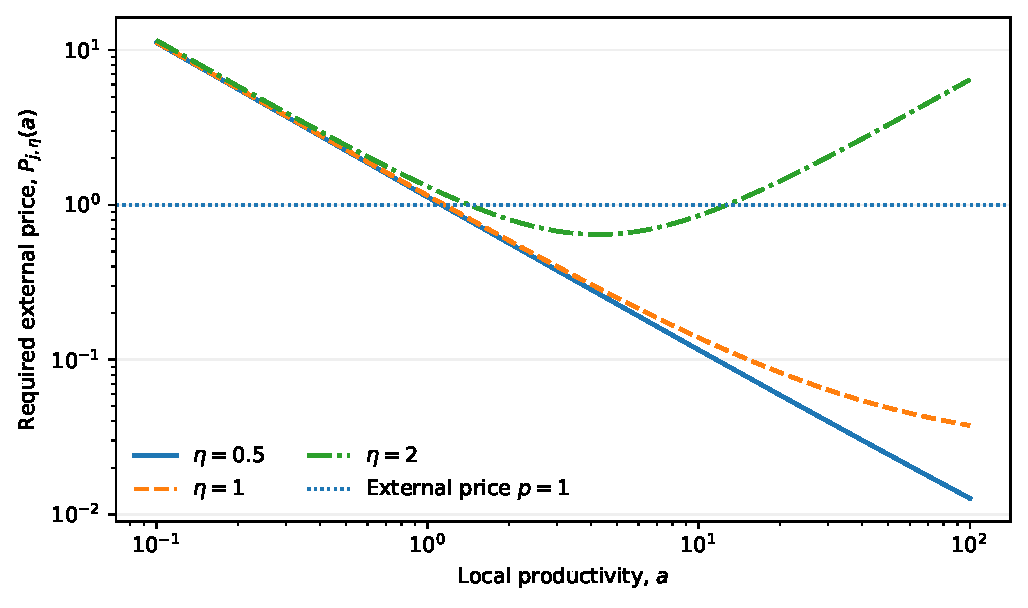
\includegraphics[width=.93\textwidth]{curvature.pdf}
\caption{Required external price as a function of productivity in the
curvature example. Inwardness requires the curve to be at or below the
horizontal price. The curves are evaluations of the analytical formula,
not fitted lines.}
\end{figure}

\subsection*{Production, recursion and support horizon}
The production check compares $10\ln(1+B-x)+x$ with
$10\ln(1+B-x)+\ln(1+x)$ at $B=8,10,100$, using both derived
solutions and scalar optimization. The shared inward boundary is
$B=9$, but the interior allocations differ. The generalized production
lemma is additionally checked with logarithmic, linear and shifted
square-root local production.

The recursion identity is checked at $b=3$, $d=4$ and $c=0.7$:
$W_d=121$ and $W_{d+1}=364$; the cost ratio is $3.008264463$,
while the logarithmic value increment is $1.093543064$.
The latter approaches $\ln b$, not a multiplicative value gain.
The fixed-memory support extension gives $W=255$ and $255/256$ at
$t=50$, and $W=511$ and $511/256$ at $t=60$.

\subsection*{Static and dynamic choices can reverse in either direction}
Both cases use $B_1=10$, $p_1=p_2=r_1=r_2=1$, $C_{01}=C_{02}=1$,
$a_2=100$ and $\beta=0.9$. Case A has $a_1=100$, $B_{20}=1$,
$g_L=0.2$, $g_X=2$; case B has $a_1=5$, $B_{20}=0$,
$g_L=0.1$, $g_X=0$. In case B, the present-only maximizer is $x=6$
because $z_1^*=a_1p_1/r_1-1=4$. At the inward corner, its continuation
budget is $B_2=1$, so
\[
 D_{\rm static}=\frac{1-5/11}{2+5\ln 11},\qquad
 D_{\rm future}=-0.09\frac{100}{2(2+100\ln 2)}.
\]
The sum is negative, proving the inward two-period optimum by concavity.
The opposite signs in case A show why a static corner is not sufficient
either. The complete output is \path{results/v73_checks.json}.

\begin{table}[htbp]\centering
\caption{New checks of the two directional reversals. The terms sum to
the derivative of the full two-period objective at $x=0$.}
\label{tab:dynamic-reversals}
\begin{tabular}{@{}lrrrrr@{}}\toprule
Case & Static term & Future term & Total & Static $x^*$ & Dynamic $x^*$\\\midrule
A & -0.03346261 & +0.28799092 & +0.25452830 & 0 & 3.75591686 \\
B & +0.03899035 & -0.06310058 & -0.02411023 & 6 & 0.00000000 \\
\bottomrule\end{tabular}\end{table}

The new script reconstructs the continuation formula and checks the
endpoint or derivative-root optimum against a bounded scalar optimizer
including both endpoints. A separate SLSQP formulation optimizes
$(x_1,z_2,x_2)$ jointly, with an explicit second-period budget constraint
and three feasible initial conditions in each case. A grid also checks
the objective and the monotonicity of its derivative. These are numerical
implementation checks, not replacements for the concavity proof.

\subsection*{A lower bound for general concave local production}
Corollary~7.1 requires differentiability at $B>0$, not at the origin,
so it includes $\ell(z)=\sqrt z$. The ratios are
\[
 \frac{\ell(B)}{\ell'(B)}=
 \begin{cases}
  2B,&\ell(z)=\sqrt z,\\
  e^B-1,&\ell(z)=1-e^{-z},\\
  B,&\ell(z)=z.
 \end{cases}
\]
All meet the lower bound $B$. The code evaluates the functions and
derivatives separately and checks these identities and the supporting-line
inequality. Table~\ref{tab:general-floor} uses $S_j=0.001$.

\begin{table}[htbp]\centering
\caption{Residual-floor checks for three concave production functions.
The final column is the general lower bound, not an approximation to the
floor.}\label{tab:general-floor}
\begin{tabular}{@{}lrrrr@{}}\toprule
$\ell(z)$ & $B$ & $\ell(B)/\ell'(B)$ & $H_j^{\ell}$ & $S_jB$\\\midrule
$\sqrt z$ & 1 & 2.000000 & 0.002000000 & 0.001 \\
$\sqrt z$ & 2 & 4.000000 & 0.004000000 & 0.002 \\
$\sqrt z$ & 10 & 20.000000 & 0.020000000 & 0.010 \\
$1-e^{-z}$ & 1 & 1.718282 & 0.001718282 & 0.001 \\
$1-e^{-z}$ & 2 & 6.389056 & 0.006389056 & 0.002 \\
$1-e^{-z}$ & 10 & 22025.465795 & 22.025465795 & 0.010 \\
$z$ & 1 & 1.000000 & 0.001000000 & 0.001 \\
$z$ & 2 & 2.000000 & 0.002000000 & 0.002 \\
$z$ & 10 & 10.000000 & 0.010000000 & 0.010 \\
\bottomrule\end{tabular}\end{table}


\clearpage
\subsection*{Reproduction commands and output mapping}
From the package root, run:
\begin{verbatim}
sh reproduce.sh
\end{verbatim}
The new numerical checks run through \path{code/validate_v73.py} and
write \path{results/v73_checks.json} and their saved grids. The exact
phase transformations, arrow coordinates, and updated Figure~3 are
produced by \path{code/make_v73_phase.py}. The archive audit is rerun in
\path{results/v73_archive_recheck/}, without overwriting its retained
outputs. Figures~1, 2 and 4 and the original numerical tables are
preserved byte for byte. The source-edit and export scripts synchronize
the modular and expanded sources, and the build regenerates all three
PDFs. The release check records source, hash and compilation checks in
\path{results/v73_release_checks.json}.

\section{Scope of the source revision}
The complete revised article, the curvature and persistence propositions,
the production lemma, and the production-floor corollary with full proofs
are in
\path{manuscript/body.tex}. The human-readable
single-file LaTeX release expands the manuscript sections,
tables and bibliography. The package provides the final manuscript,
mathematical proofs, frozen inputs, numerical outputs and executable
reproduction code.
\end{document}
